\chapter{Learning Dictionaries for Multi-Channel Signals}

\section{Introduction}
Much of the literature on using convolutional dictionaries is tailored to applications with signals that only have a small number of channels (like RGB or grayscale imagery). Many of the methods designed with a small number of channels in mind do not transfer well to applications like hyperspectral imagery \cite{PURR1947} with signal measurements containing a large number of channels.

Signal measurements are not the only way to end up with a large number of channels. In a multi-layer dictionary model, the coefficients corresponding to a dictionary from one layer become the signal for the subsequent layer.  The number of channels for this signal is the number of dictionary filters from the previous layer, so if the number of filters in a layer is large, the number of channels for the subsequent layer will also be large.

This chapter presents a novel method to learn convolutional dictionaries for multi-channel signals. 
\section{Dictionary Types}
There are many ways to construct a convolutional sparse representation of a multi-channel signal. One way models can differ is if and how signal channels share dictionaries and coefficients.

For example, models with single-channel dictionaries represent the channels in the coefficients:\footnote{In this case, both $\mX$ and $\mS$ still refer to a single sample. They are capitalized because they are matrices.}
%
\begin{equation}
\mS \approx \mD\mX
\end{equation}
\begin{equation}
\mS = \begin{bmatrix} \vs_1 & \hdots & \vs_C \end{bmatrix}
\end{equation}
\begin{equation}
\mD = \begin{bmatrix} \mD_1 & \hdots & \mD_M \end{bmatrix}
\end{equation}
\begin{equation}
\mX = \begin{bmatrix} \vx_{1,1} & \hdots & \vx_{1,C} \\ \vdots & \ddots & \vdots \\ \vx_{M,1} & \hdots & \vx_{M,C} \end{bmatrix}
\end{equation}
%
where $\vs_c \in \R^{\hat{K}}$, $\mD_m \in \R^{\hat{K} \times \hat{K}}$, and $\vx_{m,c} \in \R^{\hat{K}}$, using $\hat{K}$ as the number of elements in a single channel of the signal.

Alternatively, each signal channel could be given its own dictionary model.
%
\begin{equation}
\vs_c \approx \mD_c\vx_c
\end{equation}
%
where $\vs_c \in \R^{\hat{K}}$, $\mD_c \in \R^{\hat{K} \times M\hat{K}}$, and $\vx_{c} \in \R^{M\hat{K}}$.

In both the above-mentioned cases, the models use multi-channel coefficients. For multi-layer models, this poses a problem: with each subsequent layer, the number of coefficients grows by a factor of the number of filters. Thus, the number of coefficients increases exponentially in respect to the number of layers.

This exponential growth could be dampened (though not eliminated) through the use of product dictionaries \cite{garcia2018multichannel}. In product dictionary models, correlations between channels are captured in a separate matrix $\mSS$.
%
\begin{equation}
\mS \approx \mD\mX\mSS
\end{equation}
\begin{equation}
\mS = \begin{bmatrix} \vs_1 & \hdots & \vs_C \end{bmatrix}
\end{equation}
\begin{equation}
\mD = \begin{bmatrix} \mD_1 & \hdots & \mD_M \end{bmatrix}
\end{equation}
\begin{equation}
\mX = \begin{bmatrix} \vx_{1,1} & \hdots & \vx_{1,B} \\ \vdots & \ddots & \vdots \\ \vx_{M,1} & \hdots & \vx_{M,B} \end{bmatrix}
\end{equation}
%
where $\vs_c \in \R^{\hat{K}}$, $\mD_m \in \R^{\hat{K} \times \hat{K}}$, $\vx_{m,b} \in \R^{\hat{K}}$, and $\mSS \in \R^{B \times C}$. Pursuit algorithms for product dictionaries still seek to estimate $\mX$ for fixed $\mS$, $\mD$, and $\mSS$. For dictionary learning, $\mSS$ is updated with $\mD$.

For this work, I will instead focus on multi-channel dictionaries with shared coefficients.
%
\begin{equation}
\vs \approx \mD\vx
\end{equation}
\begin{equation}
\vs = \begin{bmatrix} \vs_1 \\ \hdots \\ \vs_C \end{bmatrix}
\end{equation}
\begin{equation}
\mD = \begin{bmatrix} \mD_{1,1} & \hdots & \mD_{1,M}  \\ \vdots & \ddots & \vdots \\ \mD_{C,1} & \hdots & \mD_{C,M} \end{bmatrix}
\end{equation}
\begin{equation}
\vx = \begin{bmatrix} \vx_1 \\ \vdots \\ \vx_M \end{bmatrix}
\end{equation}
where $\vs_c \in \R^{\hat{K}}$, $\mD_{c,m} \in \R^{\hat{K} \times \hat{K}}$, and $\vx_{m} \in \R^{\hat{K}}$, again using $\hat{K}$ to represent the number of elements in one channel of the signal.
%
When extended to multi-layer dictionaries, this structure closely aligns with that of convolutional neural networks,  and the number of channels for a subsequent dictionary is the number of filters for the dictionary from the previous layer. The number of coefficients does not grow exponentially with the number of layers, but the number of channels can be large.



\section{Pursuit and Sparse Coding}
\label{section:sparse coding}
The dictionary model decomposes the signal $\vs_n$ into a dictionary $\mD$ (which generalizes to other signals) and the coefficients $\vx_n$ (which are specific to the signal $\vs_n$):
%
\begin{equation}
\vs_n \approx \mD\vx_n
\end{equation}
%
(Here the subscript $n$ specifies a particular signal and its corresponding coefficients.) A pursuit algorithm finds the coefficients $\vx_n$ corresponding to a particular signal $\vs_n$ for known dictionary $\mD$. If the number of dictionary atoms (columns) is larger than the dimension of the signal, then the number of unknowns is larger than the number of equations, and many solutions for $\vx_n$ represent $\vs_n$ equally well (at least in an $\operatorname{L}_2$ sense). Researchers and practitioners commonly either impose a sparsity constraint on the coefficients or add a coefficient $\operatorname{L}_1$ penalty to the objective function, which removes this ambiguity from the problem construction. When such a penalty or constraint is used, pursuit is sometimes called sparse coding. With the added coefficient $\operatorname{L}_1$ penalty, the pursuit optimization problem looks like this:
%
\begin{equation}\label{equation:sparse coding}
\vx_n = \arg\min_{\vx} \frac{1}{2}\|\vs_n - \mD\vx\|_2^2 + \lambda \|\vx\|_1
\end{equation}
%
where $\lambda$ is a nonnegative hyperparameter controlling how much the $\operatorname{L}_1$ norm of the coefficients is penalized. Researchers have proposed many ways to solve this problem. If the dictionary is convolutional and the number of channels is low, a standard approach is to use the Alternating Direction Method of Multipliers (ADMM) algorithm.

\section{ADMM}
\label{section:ADMM}
ADMM is a convex-optimization algorithm used to solve the optimization problem:
\begin{equation} \label{equation:ADMM}
\begin{aligned}
\minimize_{\vx,\vy} & f(\vx) + g(\vy) \\
\text{subject to } & \mA\vx + \mB\vy + \vc = \vzero 
\end{aligned}
\end{equation}
%
where $f$ and $g$ are convex functions \cite{boyd2011distributed}. (I will address how to put the sparse coding problem in this form in the next section.)

The ADMM algorithm makes use of the augmented Lagrangian, a particular expression that has a saddle point at the solution to the constrained optimization problem:
%
\begin{equation}
\L_{\rho}(\vx,\vy,\vu) = f(\vx) + g(\vy) + \vu^H(\mA\vx + \mB\vy + \vc) + \frac{\rho}{2}\|\mA\vx + \mB\vy + \vc\|_2^2
\end{equation}
%
where $\rho$ is a hyperparameter greater than zero and $\vu$ is the dual variable for the constraints.

At the saddle-point solution, the augmented Lagrangian is at a minimum in respect to $\vx$ and $\vy$, but at a maximum in respect to $\vu$.

The ADMM algorithm is an iterative search for the saddle point of the augmented Lagrangian. Each iteration consists of a primal update for $\vx$, a primal update for $\vy$, and a dual update for $\vu$:
%
\begin{equation}
\vx^{(t + 1)} = \arg\min_{\vx} \L_{\rho}(\vx,\vy^{(t)},\vu^{(t)})
\end{equation}
%
\begin{equation}
\vy^{(t + 1)} = \arg\min_{\vy} \L_{\rho}(\vx^{(t + 1)},\vy,\vu^{(t)})
\end{equation}
%
\begin{equation} \label{equation:general dual update}
\vu^{(t + 1)} = \vu^{(t)} + \rho(\mA\vx^{(t + 1)} + \mB\vy^{(t + 1)} + \vc)
\end{equation}
%
\begin{algorithm}[H] \label{algorithm:ADMM}
\SetAlgoLined
%\KwResult{Write here the result }
 %initialization:\\
   $\vy = $ initial guess \\
   $\vu = \vzero$ \\
 \While{Not Converged}{
  $\vx = \arg \min_{\vx}  \L_{\rho}(\vx,\vy,\vu)$ \\
  $\vy = \arg \min_{\vy} \L_{\rho}(\vx,\vy,\vu)$ \\
  $\vu = \vu + \rho(\mA\vx + \mB\vy + \vc)$
 }
 \caption{ADMM}
\end{algorithm}

The primal updates serve to move towards the minimum of the augmented Lagrangian in respect to $\vx$ and $\vy$ with $\vu$ fixed, and the dual update fixes $\vx$ and $\vy$, and performs gradient ascent on $\vu$ with step size $\rho$. Under very mild assumptions, this process converges to a saddle point of the augmented Lagrangian, which matches a solution to the constrained optimization problem.\footnote{Neither the saddle point nor the corresponding solution to the constrained optimization problem are guaranteed to be unique, however.} The ADMM algorithm is shown in Algorithm \ref{algorithm:ADMM}.

There are two common variations of the ADMM algorithm that this dissertation will make use of.  The first is the scaled form, which comes from completing the square for the augmented lagrangian function:
%
\begin{equation}
\L_{\rho}(\vx,\vy,\vu) = f(\vx) + g(\vy) + \frac{\rho}{2}\|\mA\vx + \mB\vy + \vc + \frac{\vu}{\rho}\|_2^2 - \frac{\rho}{2}\|\frac{\vu}{\rho}\|_2^2
\end{equation}
%
The term $-\frac{\rho}{2}\|\frac{\vu}{\rho}\|_2^2$ can be ignored for the primal updates because it has no dependence on the primal variables. It is sometimes more convenient to keep track of $\vu_{\text{sc}} = \frac{\vu}{\rho}$ instead of $\vu$, since that is the form that appears in the augmented Lagrangian after completing the square. The dual update for the scaled form is easily derived from equation \ref{equation:general dual update}.
%
\begin{equation}
\frac{\vu^{(t + 1)}}{\rho} = \frac{\vu^{(t)}}{\rho} + \mA\vx^{(t + 1)} + \mB\vy^{(t + 1)} + \vc
\end{equation}
%
This form is known as scaled ADMM.

Another common variation of ADMM updates the dual variable more frequently \cite{eckstein1994parallel}.
\begin{equation}
\vx^{(t + 1)} = \arg\min_{\vx} \L_{\rho}(\vx,\vy^{(t)},\vu^{(t)})
\end{equation}
%
\begin{equation}
\vu^{(t + \frac{1}{2})} = \vu^{(t)} + (\alpha - 1)\rho(\mA\vx^{(t + 1)} + \mB\vy^{(t)} + \vc)
\end{equation}
%
\begin{equation}
\vy^{(t + 1)} = \arg\min_{\vy} \L_{\rho}(\vx^{(t + 1)},\vy,\vu^{(t + \frac{1}{2})})
\end{equation}
%
\begin{equation}
\vu^{(t + 1)} = \vu^{(t + \frac{1}{2})} + \rho(\mA\vx^{(t + 1)} + \mB\vy^{(t + 1)} + \vc)
\end{equation}
%
When $\alpha > 1$, this is known as over-relaxation, and if $\alpha < 1$, this is known as under-relaxation.\footnote{I have elected to notate over/under relaxation differently than standard notation, but the $\alpha$ is the same, and the notations are mathematically equivalent. The standard notation does not use the first dual update, and instead includes another variable $\vh^{(t + 1)} = \mA\vx^{(t + 1)} - (1 - \alpha)(\mA\vx^{(t + 1)} + \mB\vy^{(t)} + \vc)$ and substitutes $\vh^{(t + 1)}$ for $\mA\vx^{(t + 1)}$ in the dual-update equation and the second primal-update equation. While more familiar to readers who have dealt with ADMM before, this standard notation complicates ADMM with an extra variable and obscures how the dual update and second primal update relate to the augmented Lagrangian.} $\alpha$ is always chosen to be greater than zero. In some applications, researchers have found using over-relaxation converges faster than without over-relaxation \cite{eckstein1994parallel}, but optimal choice of $\alpha$ is problem-dependent \cite{nishihara2015general}. Scaled ADMM with over-relaxation is shown in Algorithm \ref{algorithm:Scaled ADMM with Relaxation}.

\begin{algorithm}[H] \label{algorithm:Scaled ADMM with Relaxation}
\SetAlgoLined
%\KwResult{Write here the result }
 %initialization:\\
   $\alpha \in (0,2]$ \\
   $\vy = $ initial guess \\
   $\vu_{\text{sc}} = \vzero$ \\
 \While{Not Converged}{
  $\vx = \arg \min_{\vx}  \L_{\rho}(\vx,\vy,\rho\vu_{\text{sc}})$ \\
  $\vu_{\text{sc}} = \vu_{\text{sc}} + (\alpha - 1)(\mA\vx + \mB\vy + \vc)$ \\
  $\vy = \arg \min_{\vy} \L_{\rho}(\vx,\vy,\rho\vu_{\text{sc}})$ \\
  $\vu_{\text{sc}} = \vu_{\text{sc}} + \mA\vx + \mB\vy + \vc$
 }
 \caption{Scaled ADMM With Over or Under-Relaxation}
\end{algorithm}


\section{Applying ADMM to the Sparse Coding Problem}
\label{section:Applying ADMM}
Recall from section \ref{section:sparse coding}, equation \ref{equation:sparse coding} for sparse coding.
%
\begin{equation}
\vx_i = \arg\min_{\vx} \frac{1}{2}\|\vs_i - \mD\vx\|_2^2 + \lambda \|\vx\|_1
\end{equation}
%
This can be rewritten to match the ADMM form from equation \ref{equation:ADMM}:
\begin{equation} \label{equation:SC Opt Prob}
\begin{aligned}
\minimize_{\vx,\vy} & \frac{1}{2} \|\vs_i - \mD\vx\|_2^2 + \lambda\|\vy\|_1 \\
         \text{subject to } & \vy - \vx = \vzero
\end{aligned}
\end{equation}
%
Using his form, the ADMM algorithm can be used to solve the sparse coding problem, as shown in Algorithm \ref{algorithm:ADMM for Sparse Coding}. Given sufficient iterations, $\vx$ and $\vy$ will both be close to the optimal, but they may not be equal. Either can be used as an approximate solution to the sparse coding problem.

Computing the augmented Lagrangian of the convex optimization problem in expression \ref{equation:SC Opt Prob} yields the following equation:
%
\begin{equation}
\L_{\rho}(\vx,\vy,\vu) = \frac{1}{2} \|\vs_i - \mD\vx\|_2^2 + \lambda\|\vy\|_1 + \frac{\rho}{2}\|\vy - \vx + \frac{\vu}{\rho}\|_2^2 - \frac{1}{2\rho}\|\vu\|_2^2
\end{equation}
%
Starting with the $\vx$-update:
\begin{equation}
\vx^{(t + 1)} = \arg\min_{\vx} \L_{\rho}(\vx,\vy^{(t)},\vu^{(t)})
\end{equation}
%
Since the desired result is the minimizer, setting the gradient to zero and solving for $\vx$ will produce the solution.
%
\begin{equation}
\nabla_{\vx^{(t + 1)}} \L_{\rho}(\vx^{(t + 1)},\vy{(t)},\vu{(t)}) = \vzero
\end{equation}
%
\begin{equation}
\vzero = \mD^T\mD\vx^{(t + 1)} - \mD^T\vs_i + \rho\vx^{(t + 1)} - \rho\left(\vy^{(t)} + \frac{\vu^{(t)}}{\rho}\right)
\end{equation}
%
\begin{equation}
(\rho\mId + \mD^T\mD)\vx^{(t + 1)} = \mD^T\vs_i + \rho\left(\vy^{(t)} + \frac{\vu^{(t)}}{\rho}\right)
\end{equation}
%
\begin{equation}
\vx^{(t + 1)} = (\rho\mId + \mD^T\mD)^{-1}\left(\mD^T\vs_i + \rho\left(\vy^{(t)} + \frac{\vu^{(t)}}{\rho}\right)\right)
\end{equation}
%
In subsection \ref{subsection:SC xupdate}, there is a discussion of the implications of this update equation, how to compute it for cases in which the signal has a low number of channels, and the challenges it poses for signals with many channels.

If using over-relaxation\footnote{or under-relaxation}, there is a dual update:
\begin{equation}
\frac{\vu^{(t + \frac{1}{2})}}{\rho} = \frac{\vu^{(t)}}{\rho} + (\alpha - 1)(\vy^{(t)} - \vx^{(t + 1)})
\end{equation}
%
Moving on to the $\vy$-update:
\begin{equation}
\vy^{(t + 1)} = \arg\min_{\vy} \operatorname{L}_{\rho}(\vx^{(t + 1)},\vy,\vu^{(t + \frac{1}{2})})
\end{equation}
%
Excluding the terms that don't include $\vy$ yields
\begin{equation}
\vy^{(t + 1)} = \arg\min_{\vy} \lambda\|\vy\|_1 + \frac{\rho}{2}\|\vy - \vx^{(t + 1)} + \frac{\vu^{(t + \frac{1}{2})}}{\rho}\|_2^2
\end{equation}
%
This is a well-known problem, whose solution is
\begin{equation}
\vy^{(t + 1)} = \operatorname{S}_{\frac{\lambda}{\rho}}(\vx^{(t + 1)} - \frac{\vu^{(t + \frac{1}{2})}}{\rho})
\end{equation}
where $\operatorname{S}$ is the shrinkage operator:
\begin{equation}
\operatorname{S}_{b}(x) = \begin{cases} x - b & x > b \\ 0 & -b < x < b \\ x + b & x < - b \end{cases}
\end{equation}
In the case of a vector, matrix, or tensor input, the shrinkage operator is applied element by element.

Finally, the last update equation for the dual variable:
\begin{equation}
\frac{\vu^{(t + 1)}}{\rho} = \frac{\vu^{(t + \frac{1}{2})}}{\rho} + \vy^{(t + 1)} - \vx^{(t + 1)}
\end{equation}

\begin{algorithm}[H] \label{algorithm:ADMM for Sparse Coding}
\SetAlgoLined
%\KwResult{Write here the result }
 %initialization:\\
   $\alpha \in (0,2]$ \\
   $\vy = \mD^T\vs$ \\
   $\vu_{\text{sc}} = \vzero$ \\
 \While{Not Converged}{
  $\vx = \left(\rho\mId + \mD^T\mD\right)^{-1}\left(\mD^T\vs + \rho(\vy + \vu_{\text{sc}})\right)$ \\
  $\vu_{\text{sc}} = \vu_{\text{sc}} + (\alpha - 1)(\vy - \vx)$ \\
  $\vy = \operatorname{S}_{\frac{\lambda}{\rho}}(\vx - \vu_{\text{sc}})$ \\
  $\vu_{\text{sc}} = \vu_{\text{sc}} + \vy - \vx$
 }
 \caption{ADMM for Sparse Coding}
\end{algorithm}

\subsection{Exploiting Dictionary Structure for the Inverse Problem}
\label{subsection:SC xupdate}
Returning to the $\vx$ update:
\begin{equation}
\vx^{(t + 1)} = \left(\rho\mId + \mD^T\mD\right)^{-1}\left(\mD^T\vs_i + \rho\left(\vy^{(t)} + \frac{\vu^{(t)}}{\rho}\right)\right)
\end{equation}
%
For problems using a dictionary with convolutional structure, this inverse for the convolutional sparse coding problem is very structured. Exploiting this structure is important for efficient computation, because the matrix $\rho\mId + \mD^T\mD$ is a large matrix.

Writing $\mD$ in a block structure, I have
%
\begin{equation}
\mD = \begin{bmatrix}
\mD_{1,1} & \hdots & \mD_{1,M}\\
\vdots & \ddots & \vdots\\
\mD_{C,1} & \hdots & \mD_{C,M}
\end{bmatrix}
\end{equation}
%
where $\mD_{c,m}$ is a circulant matrix capturing channel $c$ of the $m^{\text{th}}$ filter of the dictionary. Circulant matrices are diagonalizable with Fourier eigenvectors:
%
\begin{equation}
\mD = \begin{bmatrix}
\F^{-1}\hat{\mD}_{1,1}\F & \hdots & \F^{-1}\hat{\mD}_{1,M}\F\\
\vdots & \ddots & \vdots\\
\F^{-1}\hat{\mD}_{C,1}\F & \hdots & \F^{-1}\hat{\mD}_{C,M}\F
\end{bmatrix}
\end{equation}
%
where $\hat{\mD}_{c,m}$ is a diagonal matrix whose elements are the discrete Fourier transform (FFT) of channel $c$ of the $m^{\text{th}}$ dictionary filter.

This sparsely banded structure is a useful form in analyzing the structure of the inverse problem:
\begin{equation}
(\rho \mId + \mD^T\mD)^{-1} = \F^{-1}(\rho\mId + \hat{\mD}^H\hat{\mD})^{-1}\F
\end{equation}
%
where
\begin{equation}
\hat{\mD} = \begin{bmatrix}
\hat{\mD}_{1,1}, & \hdots, & \hat{\mD}_{1,M}\\
\vdots & \ddots & \vdots\\
\hat{\mD}_{C,1}, & \hdots, & \hat{\mD}_{C,M}
\end{bmatrix}
\end{equation}
%
and in a slight abuse of notation, $\F$ computes the FFT separately on the coefficients for each filter.  In \cite{Bristow2013fast}, Bristow et al. observe the matrix $\rho\mId + \hat{\mD}^H\hat{\mD}$ is sparsely banded, so the inverse can be broken down into much smaller inverse problems, and one only needs to compute the inverse of an $M \times M$ matrix for every element in the signal. ($\rho\mId + \hat{\mD}^H\hat{\mD})$ is an $M \times M$ block matrix, whose blocks are diagonal.  Each submatrix collects one element from the diagonal of each of the blocks.) This inverse can be calculated in $\mathcal{O}(\hat{K}M^3)$ time.

Furthermore, the maximum rank of these submatrices is $C$, so if $C$ is small, these inverses can be computed even more efficiently using the Woodbury matrix identity or Sherman-Morrison equations \cite{vsorel2016fast} \cite{heide2015fast} \cite{wohlberg2015efficient}.

According to the Woodbury matrix identity \cite{henderson1981deriving}, for any invertible matrix $\mU$ and any matrix $\mV$:
\begin{equation}
(\mU + \mV^H\mV)^{-1} = \mU^{-1} - \mU^{-1}\mV^H(\mId + \mV\mU^{-1}\mV^H)^{-1}\mV\mU^{-1}
\end{equation}
%
So,
\begin{equation}
(\rho\mId + \hat{\mD}^H\hat{\mD})^{-1} = \frac{1}{\rho}\mId - \frac{1}{\rho}\hat{\mD}^H(\rho\mId + \hat{\mD}\hat{\mD}^H)^{-1}\hat{\mD}
\end{equation}
%
This means that instead of computing inverse of $\hat{K}$ $M \times M$ matrices (where $K$ is the number of elements in a single channel of the signal), one could instead choose to compute the inverse of $\hat{K}$ $C \times C$ matrices. Rather than computing an inverse explicitly, it is generally preferable to calculate a Cholesky or LDLT decomposition instead, and the efficiency gains due to the Woodbury matrix identity are relevant regardless of the chosen representation. The inverse or matrix decomposition can be computed in $\mathcal{O}(\hat{K}C^3)$ time.

\section{Sparse Coding for Multi-Channel Signals: Alternatives to My Novel Approach}
In applying ADMM to the convolutional sparse coding problem, \cite{vsorel2016fast} \cite{heide2015fast} \cite{wohlberg2015efficient} exploit the low-rank structure of the inverse problem in the $\vx$ update for efficient computation. Unfortunately, this relies on the number of channels being small, as the rank corresponds to the minimum of the number of channels $C$ and the number of filters $M$. Broadly, there are two main approaches to avoid or simplify this challenging inverse problem: either construct a variant of the ADMM algorithm that simplifies the inverse problem, or use a proximal gradient approach that avoids it altogether.

In \cite{chodosh2018deep}\cite{murdock2018deep}, the authors use the ADMM algorithm for sparse coding. They observe that if the dictionary is a tight frame, that is, $\mD\mD^T = \mId$, then the inverse can be simplified without using the frequency representation.
%
\begin{equation}
(\rho\mId + \mD^T\mD)^{-1} = \frac{1}{\rho}\mId - \frac{1}{\rho(\rho + 1)}\mD^T\mD
\end{equation}
%
This produces the $\vx$ update equation:
%
\begin{equation}
\vx^{(t + 1)} = \frac{1}{\rho + 1}\mD^T\vs + \left(\mId - \frac{1}{\rho + 1}\mD^T\mD\right)\left(\vz^{(t)} - \frac{\vgamma^{(t)}}{\rho}\right)
\end{equation}
%
The above equations can be derived using the Woodbury matrix identity. In their work, they use the equations built on the assumption that the dictionary is a tight frame, but develop no mechanism to ensure that their assumption is accurate. Thus, ultimately $\frac{1}{\rho}\mId - \frac{1}{\rho(\rho + 1)}\mD^T\mD$ merely serves as an approximation to $(\rho\mId + \mD^T\mD)^{-1}$. Empirically, they observe that the algorithm converges, but the dictionaries they learn are not tight frames, so the solution they converge to is not optimal\footnote{The solution does not minimize the sparse coding objective function.}.

Other works avoid the ADMM algorithm entirely.

The iterative shrinkage thresholding algorithm (ISTA) is an iterative algorithm that minimizes the sum of two convex functions $f$ and $g$. $f$ is required to be smooth. It is helpful for $f$ to be easily differentiable and $g$ to have a simple proximal operator.
%
\begin{equation}
\prox_g(\vmu) = \arg \min_{\vnu} \frac{1}{2}\|\vnu - \vmu\|_2^2 + g(\vnu)
\end{equation}
%
Then, ISTA has the following update equation, where the constant $\mathbb{L}$ controls step size.
%
\begin{equation}
\vx^{(t + 1)} = \prox_{\frac{g}{\mathbb{L}}}\left(\vx^{(t)} - \frac{1}{\mathbb{L}}\nabla_{\vx} f(\vx^{(t)})\right)
\end{equation}
%
FISTA is similar to ISTA, but adds momentum \cite{beck2009fast}.
\begin{equation}
\vz^{(t + 1)} = \prox_{\frac{g}{\mathbb{L}}}\left(\vx^{(t)} - \frac{1}{\mathbb{L}}\nabla_{\vx}f(\vx^{(t)})\right)
\end{equation}
\begin{equation}
r^{(t + 1)} = \frac{1}{2}\left(1 + \sqrt{1 + 4(r^{(t)})^2}\right)
\end{equation}
\begin{equation}
\vx^{(t + 1)} = \vz^{(t + 1)} + \frac{r^{(t)} - 1}{r^{(t + 1)}}(\vz^{(t + 1)} - \vx^{(t)})
\end{equation}
%
Applying FISTA to the sparse coding problem, $\frac{1}{2}\|\vs - \mD\vx\|_2^2$ is straightforward to differentiate and $\lambda\|\vx\|_1$ has a simple proximal operator.
%
\begin{equation}
\nabla_{\vx}\left(\frac{1}{2}\|\vs - \mD\vx\|_2^2\right) = \mD^T\mD\vx - \mD^T\vs
\end{equation}
%
\begin{equation}
\prox_{\frac{\lambda}{\mathbb{L}}\|\cdot\|_1}(\cdot) = \operatorname{S}_{\frac{\lambda}{\mathbb{L}}}
\end{equation}
%
So, the FISTA equations for convolutional basis pursuit are the following:
\begin{equation}
\vz^{(t + 1)} = \operatorname{S}_{\frac{\lambda}{\mathbb{L}}}\left(\vx^{(t)} - \frac{1}{\mathbb{L}}\mD^T(\mD\vx^{(t)} - \vs)\right)
\end{equation}
\begin{equation}
r^{(t + 1)} = \frac{1}{2}\left(1 + \sqrt{1 + 4(r^{(t)})^2}\right)
\end{equation}
\begin{equation}
\vx^{(t + 1)} = \vz^{(t + 1)} + \frac{r^{(t)} - 1}{r^{(t + 1)}}(\vz^{(t + 1)} - \vx^{(t)})
\end{equation}
%
In \cite{wohlberg2015efficient}, Wohlberg compares FISTA to ADMM on a sparse coding task and finds FISTA converges much slower than ADMM. However, the comparison is made on signals with few channels, so ADMM is able to exploit the structure of $\mD$ for efficient $\vx$ updates.

In a recent work \cite{chodosh2020use}, Chodosh and Lucey derive prox-linear updates using convex solver methods detailed in \cite{xu2013block}. The updates come from the formula:
\begin{equation}
\vz^{(t + 1)} = \arg\min_{\vz} \left(\nabla f(\vx^{(t)})\right)^T(\vz - \vx^{(t)}) + \frac{\mathbb{L}}{2}\|\vz - \vx^{(t)}\|_2^2 + \lambda\|\vz\|_1
\end{equation}
%
where $\vx^{(t)} = \vz^{(t)} + \omega^{(t)}(\vz^{(t)} - \vz^{(t - 1)})$ and $\omega^{(t)}$ is a momentum factor. This yields the update equation\footnote{In their paper, they add a non-negativity constraint and allow different $\lambda$ for the coefficients of each filter (and possibly spatially varied as well). They also are constructing the equations specifically for a multi-layer network. Those modifications relate to their objective function and constraints, not their minimization algorithm, so I rewrote their equations without those modifications to illustrate how their approach relates to the FISTA algorithm.}:
\begin{equation}
\vz^{(t + 1)} = \operatorname{S}_{\frac{\lambda}{\mathbb{L}}}\left(\vx^{(t)} - \frac{1}{\mathbb{L}}\mD^T(\mD\vx^{(t)} - \vs)\right)
\end{equation}
%
\begin{equation}
\vx^{(t + 1)} = \vz^{(t + 1)} + \omega^{(t)}(\vz^{(t + 1)} - \vz^{(t)})
\end{equation}
%
While neither Chodosh and Lucey, nor the work they cite, mention FISTA, the resemblance is very close. The only distinction is in the momentum step.  Given these similarities, it is likely the performance between the two methods is similar.

\section{Dictionary Learning}
The last few sections have focused on sparse coding. For sparse coding, the dictionary is fixed or known. Most dictionary learning algorithms alternate between pursuing coefficients and updating dictionary filters, as shown in Algorithms \ref{Algorithm: Online Dictionary Learning} and \ref{Algorithm: Batch Dictionary Learning}.\footnote{The capital $\mS$ in Algorithm \ref{Algorithm: Batch Dictionary Learning} represents the entire collection of signal samples, as opposed to a single signal $\vs$.} The CoefficientUpdate in Algorithm \ref{Algorithm: Batch Dictionary Learning} may consist of one or more sparse coding update steps. Not all dictionary learning algorithms perfectly adhere to this structure \cite{aharon2006k}, but the template covers most approaches.
\begin{algorithm}[h] 
\SetAlgoLined
%\KwResult{Write here the result }
 %initialization:\\
   $\mD = \mD_{\text{init}}$ \\
   $i = 0$
 \While{Stopping Criteria Not Met}{
  $\vs = \operatorname{GetData}(i)$ \\
  $\vx = \operatorname{Pursuit}(\mD,\vs)$ \\
  $\mD = \operatorname{DictionaryUpdate}(\mD,\vs,\vx)$ \\
  $i = i + 1$
 }
 \caption{Online Dictionary Learning Algorithm}\label{Algorithm: Online Dictionary Learning}
\end{algorithm}
\begin{algorithm}[h] 
\SetAlgoLined
%\KwResult{Write here the result }
 %initialization:\\
   $\mD = \mD_{\text{init}}$ \\
   $\mX = \mX_{\text{init}}$ \\
 \While{Stopping Criteria Not Met}{
  $\mX = \operatorname{CoefficientUpdate}(\mD,\mX,\mS)$ \\
  $\mD = \operatorname{DictionaryUpdate}(\mD,\mS,\mX)$
 }
 \caption{Batch Dictionary Learning Algorithm}\label{Algorithm: Batch Dictionary Learning}
\end{algorithm}

There are many methods to updating dictionaries: FISTA, ADMM, projected stochastic gradient descent, et cetera. Good dictionaries tend to have the following characteristics:
\begin{enumerate}
\item Good dictionaries are able to represent the data well. That is \label{item:improvement property}
\begin{equation}
\vs \approx \mD\vx
\end{equation}
for some sparse coefficients $\vx$.
\item Furthermore, it is desirable for the dictionary to be normalized.\label{item:normalized}
\begin{equation}
\sum_{c = 1}^C \|\vd_{c,m}\|_2^2 = 1
\end{equation}
where $\vd_{c,m}$ is the first column of $\mD_{c,m}$, that is, the $c^{\text{th}}$ channel of zero-padded dictionary filter $\vf_m$.
\item Specifically, convolutional dictionary filters are typically spatially or temporally constrained. \label{item:spatially constrained}
\begin{equation}
(\mId - \mT)\vd_{c,m} = \vzero
\end{equation}
(Here, $\mId - \mT$ selects the elements of $\vd_{c,m}$ that must be zero.) Generally, dictionary updates do not increase the size of the filters.
\end{enumerate}

Dictionary updates tend to improve data representation while maintaining normalization and spatial or temporal constraints.  If using ADMM for pursuit, every time the dictionary is updated, the inverse representation must be updated as well. The inverse representation can be updated more efficiently if the dictionary update is low rank, but approximating a dictionary update using a truncated singular value decomposition would forfeit characteristic \ref{item:normalized}. The next section describes a novel means to handle these challenges, with an explanation of how to efficiently update the inverse representation and a novel sparse coding method designed to handle dictionary updates that produce unnormalized dictionaries.

\section{A Novel Approach to Sparse Coding: ADMM with Low-Rank Dictionary Updates}
In this section, I present a novel approach to sparse coding for signals with a large number of channels. The approach uses the ADMM algorithm described in section \ref{section:ADMM} and will share many similarities to the standard ADMM sparse coding approach described in section \ref{section:Applying ADMM} for signals with few channels.

\subsection{Updating the Inverse Representation}

Under many circumstances, inverse representations can be updated efficiently, provided the update adheres to a low-rank structure. Recall the frequency representation of the convolutional dictionary:
%
\begin{equation}
\hat{\mD} = \begin{bmatrix}
\hat{\mD}_{1,1} & \hdots & \hat{\mD}_{1,M}\\
\vdots & \ddots & \vdots\\
\hat{\mD}_{C,1} & \hdots & \hat{\mD}_{C,M}
\end{bmatrix}
\end{equation}
%
where $\hat{\mD}_{c,m}$ is diagonal for all $c$ and $m$. Let $\hat{\mD}_{c,m}[\hat{k}]$ be the $\hat{k}^{\text{th}}$ element of the diagonal and let
%
\begin{equation}
\hat{\mD}[\hat{k}] = \begin{bmatrix}
\hat{\mD}_{1,1}[\hat{k}] & \hdots & \hat{\mD}_{1,M}[\hat{k}]\\
\vdots & \ddots & \vdots\\
\hat{\mD}_{C,1}[\hat{k}] & \hdots & \hat{\mD}_{C,M}[\hat{k}]
\end{bmatrix}
\end{equation}
%
Then $\hat{\mD}[\hat{k}]$ is a $C \times M$ matrix collecting the $\hat{k}^{\text{th}}$ frequency of all channels and filters of $\mD$. Thus, $(\rho\mId + \hat{\mD}^H\hat{\mD})^{-1}$ really consists of $\hat{K}$ separate inverse problems: $(\rho\mId + \hat{\mD}^H[\hat{k}]\hat{\mD}[\hat{k}])^{-1}$.

Consider the update equation.
%
\begin{equation}
\hat{\mD}[\hat{k}]^{(n + 1)} = \hat{\mD}[\hat{k}]^{(n)} + \hat{\mU}\hat{\mV}[\hat{k}]^H
\end{equation}
%
where $\hat{\mU}$ is an orthogonal matrix of size $C \times 
\reflectbox{R}$ and $\hat{\mV}[\hat{k}]$ is an matrix of size $M \times 
\reflectbox{R}$.\footnote{$\hat{\mU}$ and $\hat{\mV}$ are also iteration specific, but to notate that would over-clutter the equations. For efficient, low-rank updates to the inverse representation, it is possible for both $\hat{\mU}$ and $\hat{\mV}$ to vary in respect to frequency $\hat{k}$ (instead of just $\mV$). However, most convolutional models limit spatial or temporal support of the dictionary (so that the filter size is smaller than the signal), and preventing $\mU$ from varying across frequency is part of a means to satisfy that constraint.}

Then,
%
\begin{equation} \label{equation:Inverse Representation Update}
\rho\mId + (\hat{\mD}^{(n + 1)})^H[\hat{k}]\hat{\mD}^{(n + 1)}[\hat{k}] = \rho\mId + (\mD^{(n)}[\hat{k}] + \hat{\mU}\hat{\mV}^H[\hat{k}])^H(\hat{\mD}^{(n)}[\hat{k}] + \hat{\mU}\hat{\mV}^H[\hat{k}])
\end{equation}
%
For brevity and simplicity, I will drop the notation indexing the frequency $\hat{k}$ and selecting the iteration $n$ for matrix $\hat{\mD}^{(n)}[\hat{k}]$ and simply use $\hat{\mD}$ instead. However, the reader should keep in mind the $\hat{\mD}$ here is a dense $C \times M$ matrix capturing the component of the dictionary $\mD$ for implicit frequency $\hat{k}$, only a submatrix of the sparsely banded $\hat{\mD}$ of size $\hat{K}C \times M$ from earlier in this section.
%
\begin{equation}
\rho\mId + (\hat{\mD}^{(n + 1)})^H\hat{\mD}^{(n + 1)} = \rho\mId + (\hat{\mD}^{(n)})^H\hat{\mD}^{(n)} + \hat{\mV}\hat{\mU}^H \hat{\mU}\hat{\mV}^H + \hat{\mV}\hat{\mU}^H\hat{\mD}^{(n)} + (\hat{\mD}^{(n)})^H\hat{\mU}\hat{\mV}^H
\end{equation}
%
Given that $\hat{\mU}$ is an orthogonal matrix, $\hat{\mV}\hat{\mU}^H\hat{\mU}\hat{\mV}^H$ can easily be broken into $
\reflectbox{R}$ rank-one Hermitian updates.
%
\begin{equation}
\hat{\mV}\hat{\mU}^H\hat{\mU}\hat{\mV}^H = \sum_{i = 1}^{
\reflectbox{R}} \vu_{i}^H\vu_{i}\vv_{i}\vv_{i}^H
\end{equation}
%
Similarly, $\hat{\mV}\hat{\mU}^H\hat{\mD} + \hat{\mD}^H\hat{\mU}\hat{\mV}^H$ can be broken into $
\reflectbox{R}$ Hermitian, rank-two updates:
%
\begin{equation}
\hat{\mV}\hat{\mU}^H\hat{\mD} + \hat{\mD}^H\hat{\mU}\hat{\mV}^H = \sum_{\ell = 1}^{
\reflectbox{R}} \left( \vv_i\vu_i^H\hat{\mD} + \hat{\mD}^H\vu_i\vv_i^H \right)
\end{equation}
%
%
Inverse representations can be efficiently updated if the update is Hermitian and rank one. The details of such updates are discussed in Appendix \ref{chapter:Cholesky}.

The Hermitian rank-two update consists of two rank-one terms, but the terms are not Hermitian, complicating the update process. However, this can be resolved through eigendecomposition.  
%
\begin{equation}
\vv_{i}\vu_{i}^H \hat{\mD} + \hat{\mD}\vu_{i}\vv_{i}^H = \begin{bmatrix}
\vv_{i} & \hat{\mD}^H\vu_{i} 
\end{bmatrix}
\begin{bmatrix}
\hat{\mD}^H\vu_{i} & \vv_{i}
\end{bmatrix}^H
\end{equation}
%
While matrix products are not commutative, some of the eigenvalues of matrix products are commutative.  Furthermore, for general matrices $\mA$ and $\mB$ the eigenvectors of $\mA\mB$ and $\mB\mA$ are related:
%
\begin{equation}
\mB\mA\vomega = \tau\vomega  \implies  \mA\mB\mA\vomega = \tau\mA\vomega \label{equation:eigenvector relation}
\end{equation}
%
where $\tau$ is the eigenvalue and $\vomega$ is a vector.\footnote{In equation \ref{equation:eigenvector relation}, some variables are repurposed to explain some general eigenvector relationships for matrix products. The reader should be careful not confuse $\mA$ and $\mB$ for the matrices in the ADMM constraints.}  So, if $\vomega$ is an eigenvector of $\mB\mA$, $\mA\vomega$ is an eigenvector of $\mA\mB$.
%
%
\begin{equation}
\begin{bmatrix}
\hat{\mD}^H\vu_{i} & \vv_{i}
\end{bmatrix}^H
\begin{bmatrix}
\vv_{i} & \hat{\mD}^H\vu_{i} 
\end{bmatrix}
 = 
\begin{bmatrix}
\vu_{i}^H\hat{\mD}\vv_{i} & \vu_{i}^H\hat{\mD}\hat{\mD}^H\vu_{i} \\
\vv_{i}^H\vv_{i}    & \vv_{i}^H\hat{\mD}^H\vu_{i}
\end{bmatrix}
\end{equation}
%
The eigenvalues and corresponding eigenvectors of a $2 \times 2$ matrix can be computed using the quadratic formula. Assuming that the $2 \times 2$ matrix has $2$ distinct eigenvalues, the expressions for these are below.\footnote{It is not guaranteed the $2 \times 2$ matrix will have $2$ distinct eigenvalues. In Appendix \ref{chapter:eigenedge}, I consider those cases.}
%
\begin{equation}
\operatorname{eigval}\left(\begin{bmatrix} a & b \\ c & a^* \end{bmatrix}\right) = \operatorname{real}(a) \pm \sqrt{bc - (\operatorname{imag}(a))^2}
\end{equation}
%
\begin{equation}
\operatorname{eigvec}\left(\begin{bmatrix} a & b \\ c & a^* \end{bmatrix}\right) = \begin{bmatrix} b \\ -j\operatorname{imag}(a) \pm \sqrt{bc - (\operatorname{imag}(a))^2}\end{bmatrix}
\end{equation}
%
For the sake of brevity, I will drop the subscripts for $\vu$ and $\vv$.

Letting $\eta_{\vu} = \|\hat{\mD}^H\vu\|_2^2$, $\eta_{\vv} = \|\vv\|_2^2$, and $\eta_{\vu,\vv} = \vu^H\hat{\mD}\vv$:
%
\begin{equation}
\operatorname{eigval}\left(\begin{bmatrix}
\eta_{\vu,\vv} & \eta_{\vu} \\
\eta_{\vv}    & \eta_{\vu,\vv}^*
\end{bmatrix}\right)
= \operatorname{real}(\eta_{\vu,\vv}) \pm \sqrt{\eta_{\vv}\eta_{\vu} - (\operatorname{imag}(\eta_{\vu,\vv}))^2}
\end{equation}
%
\begin{equation}
\operatorname{eigvec}
\left(\begin{bmatrix}
\eta_{\vu,\vv} & \eta_{\vu} \\
\eta_{\vv}    & \eta_{\vu,\vv}^*
\end{bmatrix}\right)
= \begin{bmatrix}
\eta_{\vu} \\
-j\operatorname{imag}(\eta_{\vu,\vv}) \pm \sqrt{\eta_{\vv}\eta_{\vu} - (\operatorname{imag}(\eta_{\vu,\vv}))^2}
\end{bmatrix}
\end{equation}
%
%
%
Therefore, 
%
\begin{equation}
\operatorname{eigvec}
(
\vv\vu^H\hat{\mD} + \hat{\mD}^H\vu\vv^H
) = 
\eta_{\vu}\vv +
\left(-j\operatorname{imag}(\eta_{\vu,\vv}) \pm \sqrt{\eta_{\vv} \eta_{\vu} - (\operatorname{imag}(\eta_{\vu,\vv}))^2}\right)\hat{\mD}^H\vu
\end{equation}
%
%
\begin{equation}
\operatorname{eigval}(
\vv\vu^H\hat{\mD} + \hat{\mD}^H\vu\vv^H
)
= \operatorname{real}(\eta_{\vu,\vv}) \pm \sqrt{\eta_{\vv}\eta_{\vu} - (\operatorname{imag}(\eta_{\vu,\vv}))^2}
\end{equation}
%
Assuming that the matrix is diagonalizable and that the eigenvectors are orthonormal,\footnote{This is not guaranteed. See appendix B for details.} if $\tau_+$ and $\tau_-$ are the eigenvalues of $\vv\vu^H\hat{\mD} + \hat{\mD}^H\vu\vv^H$ and $\vomega_+$ and $\vomega_-$ are the corresponding eigenvectors, then 
\begin{equation}
\vv\vu^H\hat{\mD} + \hat{\mD}^H\vu\vv^H = \tau_+\vomega_+\vomega_+^H + \tau_-\vomega_-\vomega_-^H
\end{equation}
So, the rank-$2$ updates can be split into $2$ rank-$1$ components that can be used to update the inverse representation for $\rho\mId + \hat{\mD}^H[\hat{k}]\hat{\mD}[\hat{k}]$.
Therefore, the update from equation \ref{equation:Inverse Representation Update}
\begin{equation}
\rho\mId + (\hat{\mD}^{(n + 1)})^H[\hat{k}]\hat{\mD}^{(n + 1)}[\hat{k}] = \rho\mId + (\mD^{(n)}[\hat{k}] + \hat{\mU}\hat{\mV}^H[\hat{k}])^H(\hat{\mD}^{(n)}[\hat{k}] + \hat{\mU}\hat{\mV}^H[\hat{k}])
\end{equation}
consists of $3\reflectbox{R}$ rank-$1$ Hermitian updates, and the updates must be computed for each frequency $\hat{k}$. Appendix A explains how to update a Cholesky decomposition with rank-$1$ Hermitian updates.

Recall once again, the dictionary update under consideration:
\begin{equation}
\hat{\mD}^{(n + 1)}[\hat{k}] = \hat{\mD}^{(n)}[\hat{k}] + \hat{\mU}\hat{\mV}^H[\hat{k}]
\end{equation}
%
This update must be of rank $\reflectbox{R}$ at every frequency. Furthermore, the dictionary filter is spatially or temporally limited to its filter size. This second constraint is met if $\hat{\mV}^H[\hat{k}]$ is similarly spatially limited.

\subsection{Computational Cost}
Given an updated dictionary $\mG^{(n + 1)}$ from some standard dictionary learning update, directly computing the Cholesky decomposition of $\rho\mId + \left(\hat{\mG}^{(n + 1)}\right)^H\hat{\mG}^{(n + 1)}$ is of computational cost $\bigO(\hat{K}M^3)$.\footnote{With the use of the Woodbury matrix lemma, this can be instead computed in $\bigO(\hat{K}C^3)$.} The novel approach for the inverse update presented in the previous section replaces the direct computation with low-rank updates to the Cholesky decomposition. This involves two steps:
\begin{enumerate}
\item
Approximate a standard dictionary update with a low-rank approximation: $\hat{\mU}\hat{\mV}[\hat{k}]^H \approx \hat{\mG}^{(n + 1)}[\hat{k}] - \mR\hat{\mD}^{(n)}[\hat{k}]$
\item
Use the low-rank approximation to update the Cholesky decomposition of $\rho\mId + (\mR\hat{\mD})^H\mR\hat{\mD}$.
\end{enumerate}

Since $\hat{\mU}$ does not vary with frequency, the first step can be computed in spatial domain. Just as in the frequency domain, the bracket indexing indicates $\mG[k]$ is a $C \times M$ matrix, corresponding to $k^{\text{th}}$ element for each filter and channel.
\begin{equation}
\mU,\mSigma,\mV_{\text{normalized}} = \operatorname{SVD}\left(\begin{bmatrix}\mG^{(n + 1)}[0] - \mR\mD^{(n)}[0] & \cdots & \mG^{(n + 1)}[K] - \mR\mD^{(n)}[K]    \end{bmatrix}\right)
\end{equation}
\begin{equation}
\mV = \mV_{\text{normalized}}\mSigma
\end{equation}

In many applications, the filter size $K$ will be much smaller than the signal size $\hat{K}$.  The computational cost of this operation is $\bigO(C^2KM) + \bigO(CM\hat{K}\operatorname{log}(\hat{K}))$. Replacing the SVD computation with a randomized SVD reduces the computational cost even further $\bigO(\reflectbox{R}CKM) + \bigO(CM\hat{K}\operatorname{log}(\hat{K}))$.

The second step applies $3\reflectbox{R}$ rank-$1$ Hermitian updates to the Cholesky decomposition. Each update can be computed in $\bigO(\hat{K}M^2)$ time.\footnote{Similar to in the direct computation case, the Woodbury matrix lemma can be used to replace the $M^2$ with $C^2$ in the computational complexity. However, it is important to account for the fact that $\hat{\mV}$ is not an orthogonal matrix, since it loses its orthogonality in the Fourier transform. (A unitary transform applied to the columns of a matrix whose rows are orthogonal does not necessarily preserve that orthogonality.) Fortunately, $\hat{\mV}^H[\hat{k}]\hat{\mV}[\hat{k}]$ can be diagonalized in $\bigO(M\reflectbox{R}^2)$ time using the eigendecomposition, which can subsequently be used to diagonalize $\hat{\mU}\hat{\mV}^H\hat{\mV}\hat{\mU}$ in $\bigO(C\reflectbox{R}^2$. Since this must be done for each frequency, these diagonalizations would require $\bigO(M\reflectbox{R}^2\hat{K}) + \bigO(C\reflectbox{R}^2\hat{K})$.}  

So, the dictionary update computational cost for this novel approach requires $\bigO(\reflectbox{R}CKM) + \bigO(CM\hat{K}\operatorname{log}(\hat{K})) + \bigO(\reflectbox{R}\hat{K}M^2)$.\footnote{If $C$ is smaller than $M$, this computational complexity can be reduced using the Woodbury matrix lemma.}

Using filter size $K = 5$ and signal size $\hat{K} = 64$, I compared the update times of the full Cholesky decomposition from scratch to the Cholesky update described in the previous section. For this comparison, I used a rank-$1$ approximation $\reflectbox{R} = 1$ and kept the number of filters equal to the number of channels $M = C$. Computations were computed on a CPU. The results are shown in Figure \ref{Figure:Computational Comparison}. For a large number of channels and filters, the computation time for directly computing the Cholesky decomposition from scratch exceeds the computation time for updating a previous decomposition.

\begin{figure}
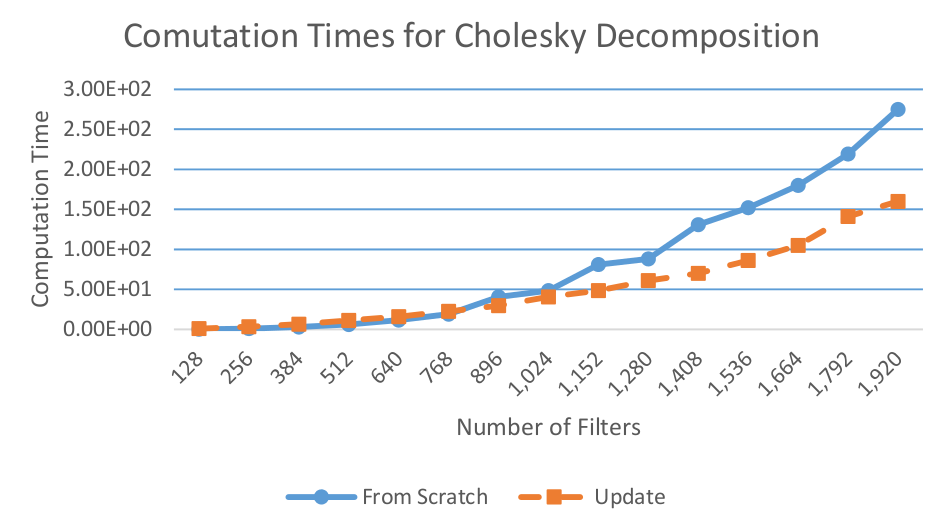
\includegraphics[width=\textwidth]{figures/computationtimes.png}
\caption{This plot shows a comparison of computation times for computing the Cholesky decompostion directly versus updating it instead. In all runs, the number of channels is the same as the number of filters.}
\label{Figure:Computational Comparison}
\end{figure}


\subsection{Handling Dictionary Normalization}
Consider the optimization problem:
%
\begin{equation}
\begin{aligned}
\min_{\vx,\vy} & \frac{1}{2}\|\vs -\mD\vx\|_2^2 + \lambda\|\vy\|_1 \\
\text{subject to } & \mR^{-1}\vy - \mR^{-1}\vx = 0 
\end{aligned}
\end{equation}
%
where $\mR$ is a diagonal matrix with scaled identity blocks:
%
\begin{equation}
\mR = \begin{bmatrix} r[1]\mId & \vzero & \hdots & \vzero \\ \vzero & r[2]\mId &  & \vdots \\ \vdots &  & \ddots &   \\ \vzero & \hdots &  & r[M]\mId \end{bmatrix}
\end{equation}
%
and $\mD$ has normalized dictionary filters.

This optimization problem has the augmented Lagrangian function:
%
\begin{equation}
\L_{\rho}(\vx,\vy,\vu) = \frac{1}{2}\|\vs - \mD\vx\|_2^2 + \lambda\|\vy\|_1 + \vu^H\mR^{-1}(\vy - \vx)  + \frac{\rho}{2}\|\mR^{-1}(\vy - \vx)\|_2^2
\end{equation} 
%
\begin{equation}
\nabla_{\vx}\operatorname{L}_{\rho}(\vx,\vy,\vu) = -\mR^{-1}\vu - \mD^H\vs + \mD^T\mD\vx + \rho\mR^{-2}\vx - \rho\mR^{-2}\vy
\end{equation}
%
For $\vx,\vy,\vu$ such that $\nabla_{\vx}\L_{\rho}(\vx,\vy,\vu) = 0$:
%
\begin{equation}
(\rho\mR^{-2} + \mD^T\mD)\vx = \rho\mR^{-2}\vy + \mR^{-1} \vu + \mD^T\vs
\end{equation}
%
\begin{equation}
\mR^{-1}\left(\rho\mId + (\mD\mR)^T(\mD\mR)\right)\mR^{-1}\vx = \rho\mR^{-2}\vy + \mR^{-1}\vu + \mD^T\vs
\end{equation}
%
\begin{equation}
\left(\rho\mId + (\mD\mR)^T(\mD\mR)\right)\mR^{-1}\vx = \rho\mR^{-1}\vy + \vu + (\mD\mR)^T\vs
\end{equation}
%
\begin{equation}
\mR^{-1}\vx = \left(\rho\mId + (\mD\mR)^H(\mD\mR)\right)^{-1}\left(\rho\mR^{-1}\vy + \vu + (\mD\mR)^T\vs\right)
\end{equation}
%
So,
%
\begin{equation}
\arg\min_{\vx} \L_{\rho}(\vx,\vy,\vu) = \mR\left(\rho\mId + (\mD\mR)^T(\mD\mR)\right)^{-1}\left(\rho\mR^{-1}\vy + \vu + (\mD\mR)^T\vs\right)
\end{equation}
%
However, taking a similar approach to that of scaled ADMM, it will be simpler to track $\vs_{\text{sc}} = \mR^{-1}\vx$ instead of $\vx$ directly.
%
\begin{equation}
\mR^{-1}\vx^{(t + 1)} = \left(\rho\mId + (\mD\mR)^T(\mD\mR)\right)^{-1}\left((\mD\mR)^T\vs + \rho\left(\mR^{-1}\vy^{(t)} + \frac{\vu^{(t)}}{\rho}\right)\right)
\end{equation}
%
Moving on to the $\vy$ update,
%
\begin{equation}
\arg\min_{\vy} \L_{\rho}(\vx,\vy,\vu) = \operatorname{S}_{\frac{\lambda\mR^2}{\rho}}\left(\vx - \frac{\mR\vu}{\rho}\right)
\end{equation}
%
Like with $\vx$, it is simpler to track $\vy_{\text{sc}} = \mR^{-1}\vy$ than $\vy$ itself.
%
\begin{equation}
\mR^{-1}\vy^{(t + 1)}= \operatorname{S}_{\frac{\lambda\mR}{\rho}}\left(\mR^{-1}\vx^{(t + 1)} - \frac{\vu^{\left(t + \frac{1}{2}\right)}}{\rho}\right)
\end{equation}
%
Finally, tracking $\vu_{\text{sc}} = \frac{\vu}{\rho}$ instead of $\vu$, the dual updates are 
\begin{equation}
\frac{\vu^{\left(t + \frac{1}{2}\right)}}{\rho} = \frac{\vu^{(t)}}{\rho} + (\alpha - 1)(\mR^{-1}\vy^{(t)} - \mR^{-1}\vx^{(t + 1)})
\end{equation}
%
\begin{equation}
\frac{\vu^{(t + 1)}}{\rho} = \frac{\vu^{\left(t + \frac{1}{2}\right)}}{\rho} + \mR^{-1}\vy^{(t + 1)} - \mR^{-1}\vx^{(t + 1)}
\end{equation}
%
Thus, with this modification to the sparse coding optimization problem, the inverse representation used in the $\vx$ updates can be updated efficiently (given that the dictionary updates adhere to a particular low-rank structure), and normalization can be handed through a normalization factor $\mR^{-1}$. The resulting pursuit algorithm is shown in Algorithm \ref{algorithm:ADMM for Sparse Coding, Large C}. The same pursuit algorithm in the larger dictionary learning context is shown in Algorithm \ref{Algorithm:Dictionary Learning, Using ADMM with large C}.


\begin{algorithm}[h]
\SetAlgoLined 
 %initialization:\\
   $\alpha \in (0,2]$ \\
   $\mD_{\text{sc}} = \mD\mR$  \\
   $\vy_s = \mR^{-2}\mD_{\text{sc}}^T\vs$ \\
   $\vu_s = \vzero$ \\
 \While{Not Converged}{
  $\vx_{\text{sc}} = \left(\rho\mId + \mD_{\text{sc}}^T\mD_{\text{sc}}\right)^{-1}\left(\mD_{\text{sc}}^T\vs + \rho\left(\vy_{\text{sc}} + \vu_{\text{sc}}\right)\right)$ \\
  $\vu_{\text{sc}} = \vu_{\text{sc}} + (\alpha - 1)(\vy_{\text{sc}} - \vx_{\text{sc}})$ \\
  $\vy_{\text{sc}} = \operatorname{S}_{\frac{\lambda\mR}{\rho}}(\vx_{\text{sc}} - \vu_{\text{sc}})$ \\
  $\vu_{\text{sc}} = \vu_{\text{sc}} + \vy_{\text{sc}} - \vx_{\text{sc}}$
 }
  $\vx = \mR\vx_{\text{sc}}$ \\
  $\vy = \mR\vy_{\text{sc}}$
 \caption{ADMM for Sparse Coding, Large Number of Channels}\label{algorithm:ADMM for Sparse Coding, Large C}
\end{algorithm}

\begin{algorithm}[h]
\SetAlgoLined
 %initialization:\\
   \tcp{Initialization:}
   $\alpha \in (0,2]$ \\
   $\mD\mR = \mD_{init}$ \\
   \For{$m \in \{1,\hdots M\}$}{
      $\mR_{m,m} = \|(\mD\mR)_m\|_F$
   }
   $\left(\rho\mId + \mR\mD^T\mD\mR\right) = \operatorname{ComputeDecomp}\left(\rho,\mD\mR \right)$ \\
   $i = 0$ \\
   \While{Stopping Criteria Not Met}{
   $\vs = \operatorname{GetData}(i)$ \\
   $i = i + 1$ \\
   \tcp{Pursuit:}
   $\mD_{\text{sc}} = \mD\mR$  \\
   $\vy_{\text{sc}} = \mR^{-2}\mD_{\text{sc}}^T\vs$ \\
   $\vu_{\text{sc}} = \vzero$ \\
 \While{Not Converged}{
  $\vx_{\text{sc}} = \left(\rho\mId + \mR\mD^T\mD\mR\right)^{-1}\left(\mD_{\text{sc}}^T\vs + \rho\left(\vy_{\text{sc}} + \vu_{\text{sc}}\right)\right)$ \\
  $\vu_{\text{sc}} = \vu_{\text{sc}} + (\alpha - 1)(\vy_{\text{sc}} - \vx_{\text{sc}})$ \\
  $\vy_{\text{sc}} = \operatorname{S}_{\frac{\lambda\mR}{\rho}}(\vx_{\text{sc}} - \vu_{\text{sc}})$ \\
  $\vu_{\text{sc}} = \vu_{\text{sc}} + \vy_{\text{sc}} - \vx_{\text{sc}}$
 }
  $\vx = \mR\vx_{\text{sc}}$ \\
  $\vy = \mR\vy_{\text{sc}}$  \\
   \tcp{Updating the Dictionary:} 
   $\tilde{\mD} = \operatorname{StandardDictionaryUpdate}(\mD,\mS,\mX)$ \\
   $\tilde{\mD} = \operatorname{Normalize}(\tilde{\mD})$ \\
   $\mDelta\mD = \operatorname{LowRankApprox}(\tilde{\mD} - \mD\mR)$ \\
   $\mD\mR = \mD\mR + \mDelta\mD$ \\
   \For{$m \in \{1,\hdots M\}$}
   {
      $\mR_{m,m} = \|(\mD\mR)_m\|_F$ 
   }
   $\left(\rho\mId + \mR\mD^T\mD\mR\right) = \operatorname{UpdateDecomp}\left(\left(\rho\mId + \mR\mD^T\mD\mR\right),\rho,\mD_{\text{sc}},\mDelta\mD \right)$
}
 \caption{Dictionary Learning, Using ADMM with Large Number of Channels}\label{Algorithm:Dictionary Learning, Using ADMM with large C}
\end{algorithm}


\section{Conclusion}
In this chapter, I have derived a novel sparse coding algorithm for signals with a large number of channels. One of the steps in the iterative algorithm involves solving an inverse problem, but the optimization is constructed such that the representation of the inverse can be updated efficiently $\bigO(\reflectbox{R}CKM) + \bigO(CM\hat{K}\operatorname{log}(\hat{K})) + \bigO(\reflectbox{R}\hat{K}M^2)$ when used within a dictionary-learning algorithm. For certain problems with a large number of channels, this is an improvement to existing methods, whose inverse updates require cubic complexity $\mathcal{O}(\hat{K}M^3)$.
% This is a figure in landscape orientation
%\begin{sidewaysfigure}
%\includegraphics[width=\textwidth]{figures/exampleFigure.png}
%\caption{This is another example Figure, rotated to landscape orientation.}
%\label{LandscapeFigure}
%\end{sidewaysfigure}
